\begin{frame}{Introduction: Distributed Version Control Systems}
  \begin{columns}
    \begin{column}{0.5\textwidth}
      \begin{figure}
        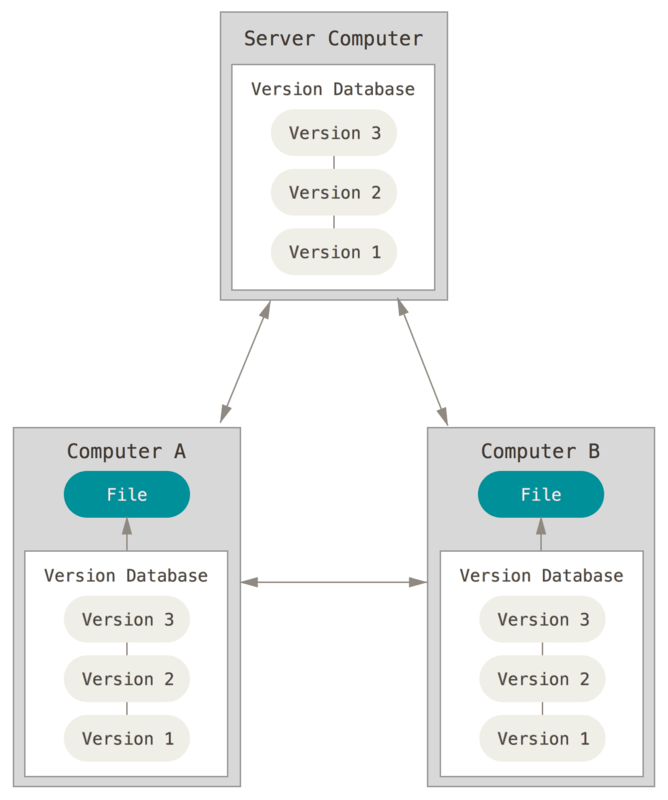
\includegraphics[width=\textwidth]{intro/distributed}
        \caption{Distributed version control}
      \end{figure}
    \end{column}
    \begin{column}{0.5\textwidth}
      Fully mirror the repository
      \footnotesize
      \begin{itemize}
        \item Recovery
        \begin{flushleft}
If any server dies, and these systems were collaborating via that server, any
of the client repositories can be copied back up to the server to restore it.
        \end{flushleft}
        \item Collaboration
        \begin{flushleft}
You can collaborate with different groups of people in different ways
simultaneously within the same project.
        \end{flushleft}
      \end{itemize}
    \end{column}
  \end{columns}
\end{frame}
